\subsection{Требования к проектируемому программному средству}
\label{sec:analysis:specification}

По результатам изучения предметной области и обзора существующих систем-аналогов сформулируем требования к проектируемому программному средству.

\subsubsection{} Назначение проекта
\label{sec:analysis:specification:purpose}

Назначением проекта является разработка программного средства, упрощающего основные задачи слежения за финансами пользователя. Приложение должно быть интуитивно понятным, а скорость взаимодействия должна быть максимальной.

\subsubsection{} Основные функции
\label{sec:analysis:specification:functions}

Программное средство должно поддерживать следующие основные фун\-к\-ции:

\begin{itemize}
	\item работа с категориями (создание, изменение, удаление, выбор типа, валюты, названия);
	\item добавление операции в категории;
	\item уведомление пользователя о приближении к заданному порогу трат;
	\item вывод статистики по категориям;
	\item очистка статистики за последний месяц в каждом новом месяце.
\end{itemize}

\subsubsection{} Требования к входным данным
\label{sec:analysis:specification:inputs}

Входные данные для программного средства должны быть представлены в виде вводимого пользователем с помощью клавиатуры текста и выбора доступных опций интерфейса чата приложения Telegram.

Должны быть реализованы проверки вводимых данных на корректность с отображением информации об ошибках в случае их некорректности.

\subsubsection{} Требования к выходным данным
\label{sec:analysis:specification:outputs}

Выходные данные программного средства должны быть представлены посредством отображения информации с помощью различных элементов интерфейса чата приложения Telegram.

\subsubsection{} Требования к временным характеристикам
\label{sec:analysis:specification:timing}

Производительность программно-аппаратного комплекса должна обеспечивать следующие временные характеристики: время реакции не запрос пользователя не должно превышать 1 секунды при минимальной скорости соединения 1 МБит/с. Допускается невыполнение данного требования в случае, когда невозможность обеспечить заявленную производительность обусловлена объективными внешними причинами.

\subsubsection{} Требования к аппаратному обеспечению серверной части
\label{sec:analysis:specification:server_requirments}

ЭВМ, на которой должна функционировать серверная часть программного средства, должна обладать следующими минимальными характеристиками:

\begin{itemize}
	\item процессор Intel Core i5 с тактовой частотой 2 ГГц;
	\item жесткий диск объемом 100 Гб;
	\item оперативная память 4 Гб;
	\item сетевая карта Ethernet 100 МБит/с.
\end{itemize}

Telegram Bot API требует наличия шифрованного HTTPS соединения, которое может быть обеспечено бесплатными утилитами, либо установкой дополнительного ПО наподобие Nginx.

% \subsubsection{} Выбор технологий программирования
% \label{sec:analysis:specification:language}

% В качестве платформы была выбрана среда .NET Core.

% .NET Core является частью .NET Foundation, который существует для построения сообщества и внедрения инноваций в рамках развития фреймворка .NET Core.

% Использование этой платформы имеет много преимуществ: разработчик получает больше свободы в контроле и изменениях проекта, прозрачность кода может снабдить информацией и послужить вдохновением для собственных проектов на базе .NET Core.

% Статус «открытости» также дает .NET Core большую устойчивость, поскольку в отличие от проприетарного программного обеспечения, которое часто бывает заброшено создателями, код, лежащий в основе инструментов этой платформы, всегда будет оставаться общедоступным.

% В связи с тем, что проект был спроектирован в соответствии с принципами открытого ПО, платформа .NET Core построена с помощью около 10 000 разработчиков. Их вклад включал pull request’ы, а также отзывы обо всем: от дизайна и UX до производительности.

% Внедряя лучшие предложения и пожелания, команда разработчиков превратила .NET Core в платформу, основанную на сообществах, что делает ее более доступной и эффективной для сообщества разработчиков, чем если бы она была создана исключительно внутри компании. Платформа продолжает совершенствоваться благодаря сотрудничеству, поскольку она поддерживается сообществом .NET, Microsoft и GitHub. Разработчик имеет возможность влиять на будущее продвижение DotNet Core, работая с кодом и оставляя отзывы.

% Ключевыми характеристиками .NET Core являются:

% \begin{itemize}
% 	\item .NET runtime, которая предоставляет .NET Core основные сервисы, включая систему типов, сборщик мусора, встроенный interop и сборку;
% 	\item примитивные типы данных, типы композиции приложений и основные утилиты предоставляются набором библиотек фреймворка, также известным как «CoreFX»;
% 	\item хост приложения «Dotnet» выбирает и запускает исполняющую среду, позволяя запускать приложения .NET Core.
% \end{itemize}

% По мере разработки разработчик получает доступ к DotNet Core в качестве пакета разработки программного обеспечения .NET Core (SDK). Он включает в себя инструменты командной строки .NET Core, .NET Core и драйвер dotnet – все, что необходимо для создания приложения или библиотеки.

% Одной из определяющих особенностей .NET Core является гибкое развертывание: имеется возможность установить платформу либо как часть своего приложения, либо отдельно. С FDD ваш пакет развертывания будет меньше. Кроме того, использование дискового пространства и использование памяти на устройствах минимизируются, и можно запустить приложение .NET Core с учетом любой ОС.

% Self-contained развертывание (SCD) включает в себя все компоненты (также библиотеки DotNet Core и среду выполнения). Этот тип развертывания дает полный контроль над версией .NET Core, используемой приложением. Уникальные характеристики каждого типа развертывания гарантируют, что разработчик получит возможность развернуть приложение оптимальным способом в зависимости от конкретных потребностей.

% Одним из основных преимуществ .NET Core является кросплатформенность. Эта уникальная программная платформа уже работает на Windows, Mac OS X и Linux. Хотя это может показаться странным шагом для Microsoft, но это важно в технологическом мире, который все больше ориентируется на гибкость и сегментированность, когда дело доходит до операционных систем и платформ.

% Доступность .NET Core на других платформах, отличных от Windows, делает его лучшим кандидатом для использования всеми разработчиками, включая разработчиков Mac и Linux, а также дает всей платформе .NET возможность использовать обратную связь. Эта дополнительная обратная связь приводит к продукту, который работает лучше для всех пользователей и позволяет DotNet Core продвигать свои приложения как программно-определяемые, а не платформо-определяемые.

% В рамках кросс-совместимости платформа для разработки приложений включает в себя модульную инфраструктуру. Она выдается через NuGet, и вы можете получить доступ к пакетным функциям, а не к одной большой сборке. Разработчик имеет возможность создавать легкие приложения, содержащие только необходимые пакеты NuGet, что сделает программу безопаснее и производительнее.

% Microsoft заявляет, что средства командной строки .NET Core служат для того чтобы «все сценарии продукта могли выполняться в командной строке». Интерфейс командной строки (CLI) является основой для инструментов высокого уровня, таких как интегрированные среды разработки, которые используется для создания приложений. Подобно платформе .NET Core, CLI является кроссплатформенным, поэтому имеется возможность использовать его на любой поддерживаемой платформе. CLI .NET Core является основой для портативности приложений.

% Хотя .NET Core был разработан как кроссплатформенная версия .NET Framework с открытым исходным кодом, между ними существуют и другие отличия, которые уходят далеко за рамки этих двух ключевых свойств. Многие из этих сравнений являются результатом дизайна и новизны .NET Core. Модели приложений, основанные на технологиях Windows, не поддерживаются .NET Core, но консольные и ASP.NET модели приложений поддерживают как .NET Core, так и .NET Framework.

% API .NET Core меньше, чем в .NET Framework, но он по мере его развития он будет увеличиваться. Кроме того, .NET Core реализует только некоторые подсистемы .NET Framework, чтобы поддерживать упрощенный и гибкий дизайн платформы. Эти различия могут в какой-то мере ограничить .NET Core, однако преимущества кроссплатформенного дизайна с открытым исходным кодом перевешивают любые ограничения по мере дальнейшего расширения платформы.

% Характер этой платформы делает ее незавершенной, постоянно совершенствуемой как командой Microsoft .NET Core, так и разработчиками по всему миру. Версия .NET Core 1.1 предназначалась для обеспечения платформы большей функциональностью. Одна из предполагаемых особенностей – улучшенная поддержка API на уровне BCL. То же касается и версии 2.0: постоянное развитие. .NET Core 2.0 также поддерживает Visual Basic. Из библиотеки DotNet Standard можно реализовать ссылку на библиотеку PCL или же на другую библиотеку DotNet Standard.

% Фактор опыта использования оказал влияние на выбор системы управления базами данных для разрабатываемого приложения. СУБД MongoDB является особенно приспособленной для веб-приложений. Ее отличительной особенностью является возможность масштабируемости, а также отказоустойчивость. Основным способом взаимодействия с данной СУБД является предложенная разработчиком клиентская библиотека на языке \csharp.

% Данная документоориентированная база данных идеально подходит для разработки программного средства. Модели данных приложения были спроектированы так, что в основном требуется лишь чтение, а обновление и запись в базу происходят намного реже. Было принято решение размещения каждой из сущностей в отдельной коллекции базы данных. Преимущество MongoDB заключается в удобстве использования, отсутствию необходимости написания запросов, а также большой спектр возможностей. Расположение коллекций приложения в базе данных изображено на рисунке \ref{fig:analysis:structure:mongo}).

% \begin{figure}[!h]
% 	\centering
% 	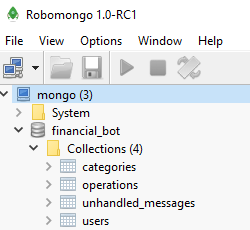
\includegraphics[scale=1]{mongodb_structure.png} 
% 	\caption{Расположение коллекций приложения в базе данных}
% 	\label{fig:analysis:structure:mongo}
% \end{figure}

% В качестве высокоуровнего API для обращения к Telegram Bot API была выбрана библиотека telegram.bot. Библиотека была выбрана, так как она предлагает наиболее полный спектр функций, поддерживаемых API Telegram. Библиотека находится в стадии активной разработки, все неисправности, выявленные пользователями, устраняются довольно быстро. К тому же, она полностью асинхронна, что позволяет снизить нагрузки на сервер во время работы.

Сформулированные требования позволят осуществить успешное проектирование и разработку программного средства.
